\documentclass[conference]{IEEEtran}
%\IEEEoverridecommandlockouts
% The preceding line is only needed to identify funding in the first footnote. If that is unneeded, please comment it out.
\usepackage{cite}
\usepackage{amsmath,amssymb,amsfonts}
\usepackage{algorithm}
\usepackage{algorithmic}
\usepackage{graphicx}
\usepackage{textcomp}
\usepackage{listings}
\usepackage{fancyvrb}
\usepackage{xcolor}
\usepackage[makeroom]{cancel}
\def\BibTeX{{\rm B\kern-.05em{\sc i\kern-.025em b}\kern-.08em
    T\kern-.1667em\lower.7ex\hbox{E}\kern-.125emX}}
\begin{document}

\title{Block Size Optimization for VBASBS Queueing Model for Blockchain}

\author{\IEEEauthorblockN{Class Project}
\IEEEauthorblockA{\textit{dept. of Computer Science} \\
\textit{Oklahoma State University}\\
Stillwater, OK, USA \\
student@okstate.edu}}

\iffalse
\author{\IEEEauthorblockN{Nathan Crosby}
\IEEEauthorblockA{\textit{dept. of Computer Science} \\
\textit{Oklahoma State University}\\
Stillwater, OK, USA \\
ncrosby@okstate.edu}

\and
\IEEEauthorblockN{Andrew Smith}
\IEEEauthorblockA{\textit{dept. of Computer Science} \\
\textit{Oklahoma State University}\\
Stillwater, OK, USA \\
scu@okstate.edu}

\and
\IEEEauthorblockN{Christopher Crick}
\IEEEauthorblockA{\textit{dept. of Computer Science} \\
\textit{Oklahoma State University}\\
Stillwater, OK, USA \\
chriscrick@cs.okstate.edu}

\and
\IEEEauthorblockN{Nohpill Park}
\IEEEauthorblockA{\textit{dept. of Computer Science} \\
\textit{Oklahoma State University}\\
Stillwater, OK, USA \\
npark@cs.okstate.edu}
}
\fi

\maketitle

\begin{abstract}

TODO: Redo this later

\end{abstract}

\begin{IEEEkeywords}
Blockchain, Optimization, Queueing
\end{IEEEkeywords}

\section{Introduction}\label{Intro}

TODO: Redo this later

\section{Related Work}\label{related}

TODO: Redo this later

\section{Methedology}
\subsection{Performance Model}\label{Model}
Our algorithm will assume the performance model proposed by Seol, Kancharla, Ke, Kim and Park
 - A Variable Bulk Arrival and Static Bulk Service Queuing Model for Blockchain\cite{2020_ACM_Seol}. 
 The arrival rate of the individual blockchain transactions is variable, but not unpredictable. 
 The arrival rate is assumed to vary with the size of the incoming transaction and the rate is 
 denoted by the symbol $\lambda$.

The variable $\mu$ is defined to be the processing time of a block to be posted and purged as noted 
in Seol\cite{2020_ACM_Seol}, and is assumed to be fairly static as stated in the model. Since this is 
assumed to be true, we will focus mainly on the performance measures of L$_Q$, W$_Q$ and $\gamma$ 
as described below.

The variable n is defined to be the total number of slots in the block. This will be used to 
define when a block (or batch of transactions) will be processed to minimize wait time while 
maximizing throughput. 

P$_i$ denotes the states with P$_n$ denoting the maximum state before the block is processed. Given 
from the paper, the performance measure L$_Q$, which is the average number of customers in the 
queue, can be written as:

\begin{equation}
L_Q=\sum_{i=0}^niP_i\label{LQ_eq}
\end{equation}

Where the equation of the sum of i times state P at i is given as:

\begin{equation}
\sum_{i=0}^niP_i=\sum_{i=0}^ni(q_iP_0(\sum_{j=1}^ij(\sum_{k=1}^{i-1}(\prod_{l=1}^{k-1}q_l)k)+i))\label{sumiPi_eq}
\end{equation}

But as can be noted from the code in the appendix of the paper which is responsible for plotting 
the associated graphs, this is equivalent to: 

\begin{equation}
\sum_{i=0}^ni(q_iP_0(\sum_{j=1}^ij(\sum_{k=1}^{i-1}(\prod_{l=1}^{k-1}q_l)k)+i))=nP_n\label{nPn_eq}
\end{equation}

Where the state P at time n is written as:

\begin{equation}
P_n=\frac{\lambda}{\mu}\frac{n(n+1)}{2}P_0\label{Pn_eq}
\end{equation}

Therefore, L$_Q$ can be written as:

\begin{equation}
L_Q=n\ast\frac{\lambda}{\mu}\frac{n(n+1)}{2}P_0\label{LQ2_eq}
\end{equation}

The performance measure W$_Q$, which is the average amount of time a customer is in the queue, 
can be written as:

\begin{equation}
W_Q=\frac{L_Q}{\lambda}\label{WQ_eq}
\end{equation}

Both of these performance measures will vary somewhat constantly by n times the ratio of 
$\frac{\lambda}{\mu}$ past some constant. And it can be noted that W$_Q$ is simply a scaled 
measure of L$_Q$. However, the opposite end of this dynamic is the throughput, or how many 
transactions will be processed in a given amount of time. This is given in the model paper as 
$\gamma$, which is the throughput of the model, and is written as:

\begin{equation}
\gamma=\mu P_n=\mu\frac{\lambda}{\mu}\frac{n(n+1)}{2}P_0=\lambda\frac{n(n+1)}{2}P_0\label{gamma_eq}
\end{equation}

These performance metrics based off of the model put forth in Seol\cite{2020_ACM_Seol} will form the basis 
of our algorithm. We will then try to minimize the waiting time while maximizing throughput based 
on the expectation of $\lambda$ to adjust n to an optimum level. In doing so, we will compare our 
non-synchronous model to a synchronous model with a set value of block size n. 

\subsection{New Model}\label{new_model}

\begin{figure*}[htbp]
    \centerline{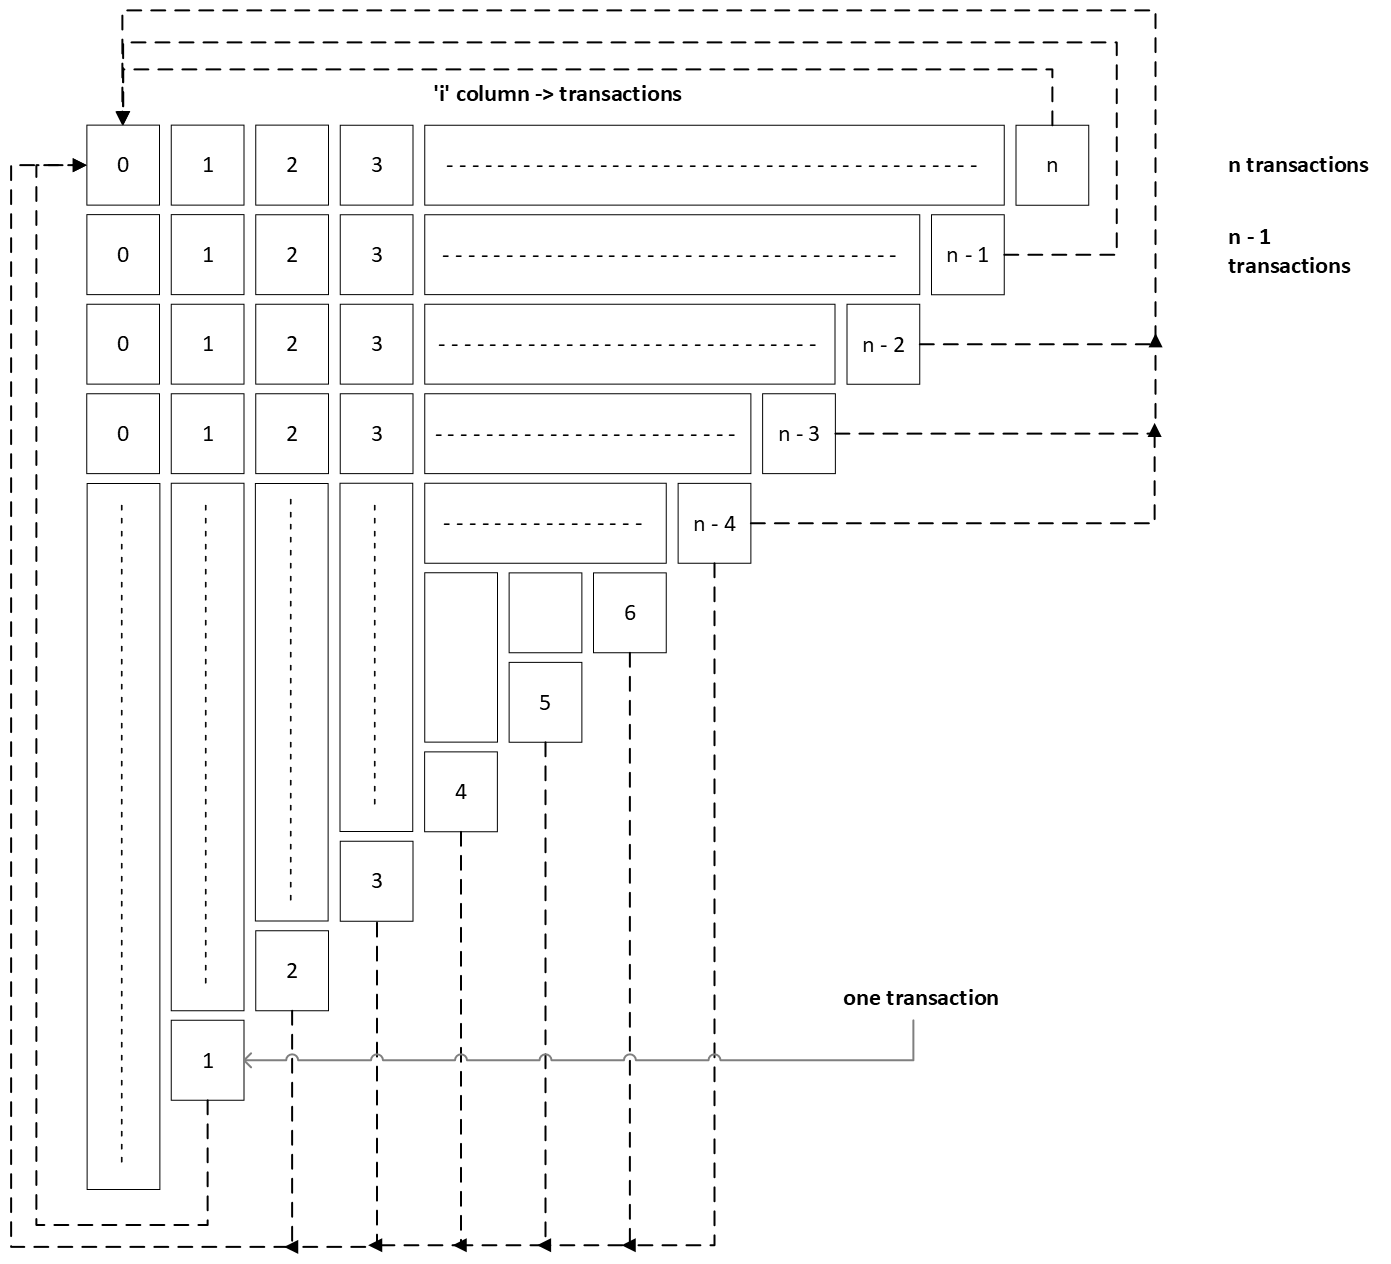
\includegraphics[width=\textwidth]{Figures/FlowDiagram.png}}
    \caption{Flow Diagram of new model.} 
    \label{flow}
\end{figure*}	

Due to the ethereum network switching from Proof of Work to Proof of
Stake validation, as discussed in Sec. ~\ref{related}, we have decided to update
the base model in Seol\cite{2020_ACM_Seol} to reflect this new regime. This 
new Proof of Stake methodology essentially flips the previous base model on its 
head, where the time between blocks being pushed out to validators is set at twelve 
seconds, and because of this, the block size (in terms of gas) can then fluctuate based 
on the number of transactions that have arrived in the latest block window of time. 

The subsequently updated variables and assumptions are given below. 

$P_{0,0}$: The state at which no time has passed in the block window of time. 

$P_{n,0}$: The state at all of the time has passed in the block window of time, and
the block is ready to be sent to the validator community, with no slow transactions. 

$P_{n-j,j}$: The state at all of the time has passed in the block window of time, and
the block is ready to be sent to the validator community, with $j$ slow transactions. 

$P_{i,0}$: The state at which $i$ fast transactions have arrived in the 
block window of time with 0 slow transactions. 

$P_{i,j}$: The state at which $i$ fast transactions have arrived in the 
block window of time with $j$ slow transactions. 

$\tau$: The number of minimum time increments that have occurred between the 
start of the block window of time and the current moment. This can be thought of
as $1/\lambda$ where $lambda$ is defined in Seol\cite{2020_ACM_Seol}.

$\Omega$: The rate for the entire block to be posted and purged. This is assumed
to balance the new form of equations as $\mu$ did in the original base model.

\subsubsection{$P_{0,0}$} $\\$

\begin{figure}[htbp]
    \centerline{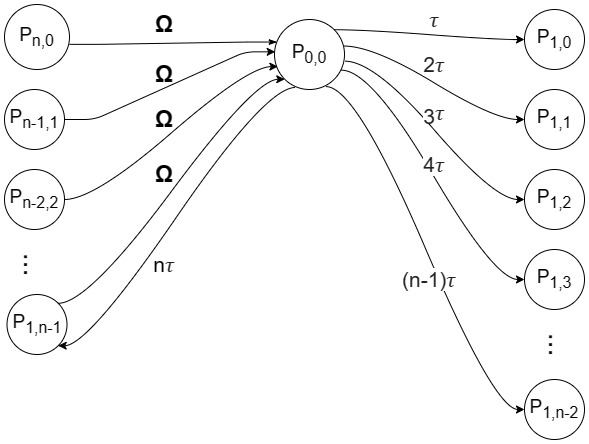
\includegraphics[width=\linewidth]{Figures/StateTransition2.jpg}}
    \caption{State Transition Diagram of $P_{0,0}$} 
    \label{trans1}
\end{figure}	

Incoming from $P_{n,0}$, $P_{n-1,1}$, $P_{n-2,2}$, ... , $P_{2,n-2}$, $P_{1,n-1}$

Outgoing to $P_{1,0}$, $P_{1,1}$, $P_{1,2}$, ... , $P_{1,n-2}$, $P_{1,n-1}$

\begin{multline}
\Omega(P_{n,0} + P_{n-1,1} + P_{n-2,2} + ... + P_{2,n-2} + P_{1,n-1})\\
= \tau(1 + 2 + 3 + ... + n-1 + n)P_{0,0}\label{nm_1}
\end{multline}

Here we have the summation from $1$ to $n-1$ which can be rewritten as 
$\frac{n(n+1)}{2}$ and the other summation is all of the possible ending states
before we return to $P_{0,0}$. This can then be rewritten in Eq. ~\ref{nm_2}.

\begin{equation}
\Omega\sum_{j=0}^{n-1}{P_{n-j,j}} = \tau\frac{n(n+1)}{2}P_{0,0}\label{nm_2}
\end{equation}

As can be seen here, our added parameter $j$ for the slow transactions has
the effect of splitting the final state, $P_n$ from the base model in 
Seol\cite{2020_ACM_Seol} into various states from $0$ slow transactions up
to $n-1$ slow transactions.

It is with this addition, along chopping a fixed amount of time to minimum time
increments, $\tau$, that we can approximate the proof of stake workflow in 
blockchain networks, like ethereum. 

\subsubsection{$P_{1,j}$} $\\$

Incoming from $P_{0,0}$ only (with time $(j+1)\tau$)

Outgoing to $P_{2,j}$, $P_{2,j+1}$, $P_{2,j+2}$, ... , $P_{2,n-3}$, $P_{2,n-2}$

\begin{multline}
\bcancel{\tau}(j+1)P_{0,0} = \\
\bcancel{\tau}(1 + 2 + 3 + ... + (n-j-2) + (n-j-1))P_{1,j}\label{nm_3}
\end{multline}

\begin{equation}
P_{0,0} = \frac{(n-j-1)(n-j)}{2(j+1)}P_{1,j}\label{nm_4}
\end{equation}

\subsubsection{Combining Eq. \ref{nm_2} and Eq. \ref{nm_4}}

\begin{multline}
\frac{\cancel{2}\Omega}{\tau (n(n+1))}(P_{n,0} + P_{n-1,1} + P_{n-2,2} + ... \\
+ P_{2,n-2} + P_{1,n-1}) = \frac{(n-j-1)(t-j)}{\cancel{2}(j+1)}P_{1,j}\label{nm_5}
\end{multline}

\begin{multline}
P_{1,j} = \frac{(j+1)\Omega}{\tau(n(n+1))((n-j-1)(n-j))}\\
(P_{n,0} + P_{n-1,1} + ... + P_{1,n-1})\label{nm_6}
\end{multline}

\subsubsection{$P_{n-j,j}$} $\\$

\begin{figure}[htbp]
    \centerline{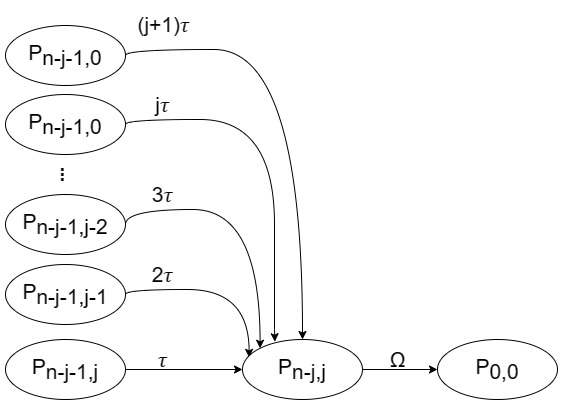
\includegraphics[width=\linewidth]{Figures/StateTransition3.jpg}}
    \caption{State Transition Diagram of $P_{n-j,j}$} 
    \label{trans2}
\end{figure}	

Incoming from $P_{n-j-1,j}$,$P_{n-j-1,j-1}$,...,$P_{n-j-1,1}$,$P_{n-j-1,0}$

Outgoing to $P_{0,0}$

\begin{multline}
\tau(P_{n-j-1,j} + 2P_{n-j-1,j-1} + 3P_{n-j-1,j-2} + ... \\
+ jP_{n-j-1,1} + (j+1)P_{n-j-1,0} = \Omega P_{n-j, j}\label{nm_7}
\end{multline}

\begin{multline}
P_{n-j, j} = \frac{\tau}{\Omega}(P_{n-j-1,j} + 2P_{n-j-1,j-1} + ... \\
+ (j+1)P_{n-j-1,0} \label{nm_8}
\end{multline}

\subsubsection{$P_{i,j}$} $\\$

\begin{figure}[htbp]
    \centerline{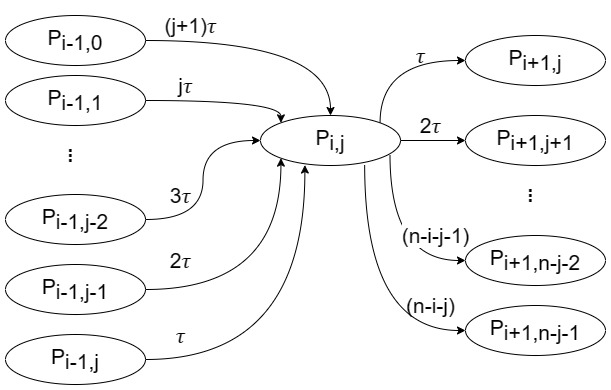
\includegraphics[width=\linewidth]{Figures/StateTransition4.jpg}}
    \caption{State Transition Diagram of $P_{i,j}$} 
    \label{trans3}
\end{figure}

Incoming from $P_{i-1,j}$, $P_{i-1,j-1}$, ... , $P_{i-1,0}$

Outgoing to $P_{i+1,j}$, $P_{i+1,j+1}$, $P_{i+1,j+2}$, ... , $P_{i+1,n-i-1}$

\begin{multline}
\bcancel{\tau}(P_{i-1,j} + 2P_{i-1,j-1} + 3P_{i-1,j-2} + ... + jP_{i-1,1} + \\
(j+1)P_{i-1,0}) = \bcancel{\tau}(1 + 2 + 3 + ... + (n-i-j-1) + \\
(n-i-j)) P_{i,j}\label{nm_9}
\end{multline}

\begin{multline}
P_{i,j} = \frac{2}{(n-i-j)(n-i-j+1)}(P_{i-1,j} + 2P_{i-1,j-1} +  \\
... + (j+1)P_{i-1,0})\label{nm_10}
\end{multline}	

\subsubsection{Constraint: Markovian Queueing Assumption}

\begin{equation}
P_{0,0} + \sum_{i=1}^{n}{\sum_{j=0}^{n-i}{P_{i,j}}} = 1.0\label{nm_11}
\end{equation}

\subsubsection{Remarks} $\\$

$\bullet$ Each $P_{i,j}$ depends on the previous $(i-1)$ column and its 
preceding $(0 ... j)$ rows. This $P_{i,j}$ in turn, affects $P_{i+1,j}$ through
$P_{i+1,n-i-1}$.

$\bullet$ The $i=0$ column has only $P_{0,0}$ (no arrivals and no time 
elapsed.

\subsection{Optimization}\label{optimization}

The main point left to discuss is the optimization problem to set n to an optimum level given what 
the new expectation is for the coming $\lambda$. The new expectation for the coming $\lambda$ will 
be the average of all $\lambda$ that we have seen up until that point, which is an unbiased estimator 
of the random variable $\lambda$ since our model will not have any prior knowledge of the range of 
values to be passed in. 
	
The derivatives of the $\gamma$ and W$_Q$ are difficult to calculate for these purposes, so to approximate 
the derivatives we will use the first differences. This calculation is given by:

\begin{equation}
\Delta \gamma = \gamma[2:n] - \gamma[1:n-1]\label{deltagamma_eq}
\end{equation}

\begin{equation}
\Delta W_Q  = W_Q [2:n] - W_Q [1:n-1]\label{deltawq_eq}
\end{equation}

Since the functions are evaluated at small, discrete, and uniformly spaced time steps the approximation 
should be accurate for our purposes. 

\begin{equation}
optN=argmin f(n):=\{ -nlg(n)\cdot\frac{\Delta \gamma}{\Delta W_Q}\}\label{optn_eq}
\end{equation}

\subsection{Closed Form Optimization}\label{closed_opt}

In this semester, we can start by removing the iterative, numerical process described above with 
a closed form solution to get the optimal n. The first thing then is that we have to look at the metric.
In the iterative process we had the ratio of throughput over waiting time multiplied by a plug of $n lg(n)$. 

Let's then look at the equations of throughput and waiting time to see how the ratio looks when reducing it 
down. W$_Q$ is given in eq. \ref{WQ_eq} as simply L$_Q$ divided by $\lambda$, so lets write that out and 
show that $\lambda$ cancels out in that equation.

\begin{equation}
W_Q=\frac{n\ast\frac{\lambda}{\mu}\frac{n(n+1)}{2}P_0}{\lambda}=n\ast\frac{\cancel{\lambda}}{\mu}\frac{n(n+1)}{2}P_0\ast\frac{1}{\cancel{\lambda}}\label{WQ_reduced}
\end{equation}

Eq. \ref{gamma_eq} gives the equation for $\gamma$, so if we look at the equation for the ratio of throughput over waiting time we get eq. \ref{ratio_eq}. 

\begin{equation}
\frac{\gamma}{W_Q}=\frac{\lambda\cancel{\frac{n(n+1)}{2}}\cancel{P_0}}{\frac{n}{\mu}\cancel{\frac{n(n+1)}{2}}\cancel{P_0}}=\frac{\lambda}{\frac{n}{\mu}}=\frac{\mu}{n}\ast\lambda\label{ratio_eq}
\end{equation}

Now, this ratio when reduced shows that throughput over waiting time is a montonically increasing function, 
with $\mu$ being fixed this means that $n$ is directly dependent on $\lambda$. This would not lead to an optimal 
level of $n$, but rather as $\lambda$ became smaller (or quicker), $n$ would should become smaller. In practice, 
batching was necessary to process transactions more efficiently, so there should be some penalty for having blocks 
that are too small. The particular network or application would probably have a direct impact on this number, but
for our case in an arbitrary blockchain, let's set this to $\frac{1}{3n^3}$. In this way, when $n$ gets very small, 
the penalty gets larger. A maximum can also be determined based on network processing speeds as a cap to 
$n$. So, now we have eq. \ref{metric_eq} which we can denote $M$ for metric.

\begin{equation}
M=\frac{\gamma}{W_Q}-penalty=\frac{\mu\lambda}{n}-\frac{1}{3n^3}\label{metric_eq}
\end{equation}

To find the maximum/minimum of this equation we need to take the first derivative with respect to $n$ 
and set it equal to zero. 

\begin{equation}
\frac{\delta M}{\delta n}=-\frac{\mu\lambda}{n^2}+\frac{1}{n^4}=0\label{metric_deriv}
\end{equation}

Then solving for $n$ we have eqs. \ref{cf_opt_n_1}, \ref{cf_opt_n_2}, \ref{cf_opt_n_3}.

\begin{equation}
-\frac{\mu\lambda}{n^2}=-\frac{1}{n^4}\label{cf_opt_n_1}
\end{equation}

\begin{equation}
\frac{n^4}{n^2}=\frac{1}{\mu\lambda}\label{cf_opt_n_2}
\end{equation}

\begin{equation}
n=\frac{1}{\sqrt{\mu\lambda}}\label{cf_opt_n_3}
\end{equation}

We now have the closed form solution that the optimal block size ($n$) is inversely related to
the square root of the cost of creating a block ($\mu$) times the speed with which the transactions 
are coming into the network($\lambda$). 

Using this same equation, $\lambda$ can also be projected based on the cyclical nature of how transaction
speeds progress throughout the day and the optimal $n$ can be calculated before each block is created to 
predetermine the next block size to be created. 

\section{Results}

TODO: Redo this later

\section{Conclusion}

TODO: Redo this later

\bibliographystyle{IEEEtrans}
\bibliography{Crosby}

\end{document}
